\subsubsection{Patch a la t�cnica The House of Mind}

Por desgracia, no todo lo bueno dura. En la versi�n 2.11 de la \textit{glibc} se corrigi� esta vulnerabilidad. Aun cuando la t�cnica de The House of Mind era tan compleja, los desarrolladores de la \textit{glibc} encontraron una soluci�n elegante al problema. El C�digo \ref{code:house_of_mind_patch} la muestra. \bigskip

\lstset{language=C, caption=Patch a The House of Mind, label=code:house_of_mind_patch}
\begin{lstlisting}
bck = unsorted_chunks(av);
fwd = bck->fd;
if (__builtin_expect (fwd->bk != bck, 0))
   {
      errstr = "malloc(): corrupted unsorted chunks";
      goto errout;
   }
\end{lstlisting}

Como se puede ver, la condici�n comprueba la integridad de la lista doblemente enlazada de \textit{unsorted chunks} de un modo parecido a como ocurr�a con la soluci�n para la vulnerabilidad \textit{unlink}. Evidentemente, al llevar a cabo The House of Mind la lista de \textit{unsorted chunks} no est� como deber�a con lo que la condici�n es verdadera y, por tanto, no se ejecuta la sobrescritura. \bigskip

Sin embargo, se deber�a realizar un estudio a fondo para contrastar si esta medida de seguridad realmente evita la ejecuci�n de la t�cnica The House of Mind. Partiendo de la base que la direcci�n del puntero |bck| y el contenido a donde apunta lo puede controlar el atacante, se hace evidente que se puede controlar la direcci�n de |bck->fd|, o sea, |fwd|. Sabiendo que |bck| apunta al primer fragmento de memoria, |bck->fd|, apunta a la direcci�n contenida en primer fragmento de memoria m�s 8 bytes. Para no cumplir la condici�n, la direcci�n contenida donde apunta |fwd| m�s 12 bytes deber�a ser igual a |bck|, o sea, igual a la direcci�n del primer fragmento de memoria. \bigskip

Un esquema gr�fico para evadir esta medida de seguridad se retrata en la Figura \ref{fig:bypass_patch}. En |bck->fd| se ha elegido poner la direcci�n del segundo fragmento de memoria simplemente porque es una regi�n de memoria de la que se pueden controlar sus contenidos. Se podr�a haber elegido cualquier otra direcci�n de la que se pudiera controlar los datos que contiene.\bigskip

\begin{figure}[!htbp]  
    \centering
    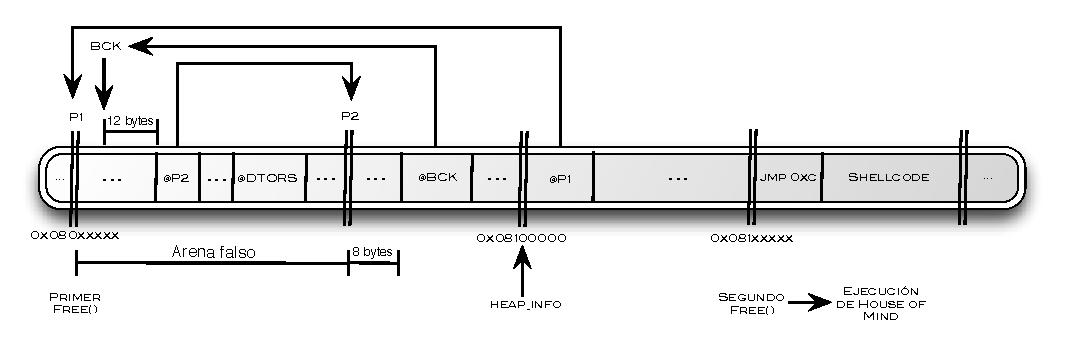
\includegraphics[scale=.85]{./Chapters/HeapExploiting/glibc/malloc_maleficarum/house_of_mind/img/bypass_patch.eps}   
    \caption{Evasi�n del patch}
    \label{fig:bypass_patch}
\end{figure}

El problema viene con que el primer fragmento de memoria simula una estructura \textit{arena}. Si en dicha estructura, ah� donde se debe escribir la direcci�n hacia la regi�n de memoria que el atacante controla, o sea si en |bck->fd| hay datos relevantes para llevar a cabo la t�cnica de The House of Mind, esta evasi�n no se podr�a levar a cabo. \bigskip

Sin embargo, cogiendo la estructura \textit{arena} en la versi�n de la \textit{glibc} 2.3.5 o la 2.12.1, si la constante |THREAD_STATS| estuviera definida, en la direcci�n |bck->fd| se sobrescribir�a el valor de una de las variables para llevar a cabo c�lculos estad�sticos |stat_lock_loop| o |stat_lock_direct|, respectivamente. Por lo tanto no tendr�a que haber ning�n problema para evadir esta medida de seguridad. \\
Si la constante |THREAD_STATS| no estuviera definida, se sobrescribir�a el array de \textit{fastbins} que, teniendo en cuenta que con esta t�cnica no se utiliza para nada, no ocasionar�a ning�n problema y, por tanto, tambi�n tendr�a que permitir la evasi�n de la medida de seguridad. 